\documentclass[hidelinks,12pt]{article}
\linespread{1.3}
\usepackage{hyperref}
\usepackage{enumerate,changepage,lipsum,titlesec, longtable}
\usepackage{cite}
\usepackage{comment, xcolor}
\usepackage[pdftex]{graphicx}
  \graphicspath{{images/}, {images/stat/}}
  \DeclareGraphicsExtensions{.pdf,.jpeg,.png, .jpg}
\usepackage[cmex10]{amsmath}
\usepackage{tikz}
\usepackage{array} 
\usepackage{subfigure} 
\newcommand{\grey}[1]{\textcolor{black!30}{#1}}
\newcommand{\red}[1]{\textcolor{red!50}{#1}}
\newcommand{\fref}[1]{Figure \ref{#1}}
\newcommand{\tref}[1]{Table \ref{#1}}

% tikz package specs
\usetikzlibrary{calc,trees,positioning,arrows,chains,shapes.geometric,%
    decorations.pathreplacing,decorations.pathmorphing,shapes,%
    matrix,shapes.symbols}

\tikzset{
>=stealth',
  punktchain/.style={
    rectangle, 
    rounded corners, 
    % fill=black!10,
    draw=black, very thick,
    text width=30em, 
    minimum height=3em, 
    text centered, 
    on chain},
  line/.style={draw, thick, <-},
  element/.style={
    tape,
    top color=white,
    bottom color=blue!50!black!60!,
    minimum width=8em,
    draw=blue!40!black!90, very thick,
    text width=10em, 
    minimum height=3.5em, 
    text centered, 
    on chain},
  every join/.style={->, thick,shorten >=1pt},
  decoration={brace},
  tuborg/.style={decorate},
  tubnode/.style={midway, right=2pt},
}

\oddsidemargin0cm
\topmargin-2cm %I recommend adding these three lines to increase the
\textwidth16.5cm %amount of usable space on the page (and save trees)
\textheight23.5cm

\makeatletter
\renewcommand\paragraph{\@startsection{paragraph}{4}{\z@}%
            {-2.5ex\@plus -1ex \@minus -.25ex}%
            {1.25ex \@plus .25ex}%
            {\normalfont\normalsize\bfseries}}
\makeatother
\setcounter{secnumdepth}{4} % how many sectioning levels to assign numbers to
\setcounter{tocdepth}{4}    % how many sectioning levels to show in ToC


\begin{document}
\title{Developing District System Design Support Package \\
       \large Computer Tool Survey and Function Specification}
\maketitle
\tableofcontents
\newpage
\section{General Introduction}
IDEA created a guide document to help planners and developers to
create energy maps. \fref{fig:energyMapIDEA} shows the contents that
could be included in energy maps: sustainable energy source (water
body, biomass, wind, hydropower) location and district heating
locations. The creation of energy maps happens after setting up the
community district energy project objectives. It involves data
collection of ``building density, mix of uses, and anchor loads''\cite
{IDEA2012} and data assembling and map creation.

\begin{figure}[h!]
  \centering
  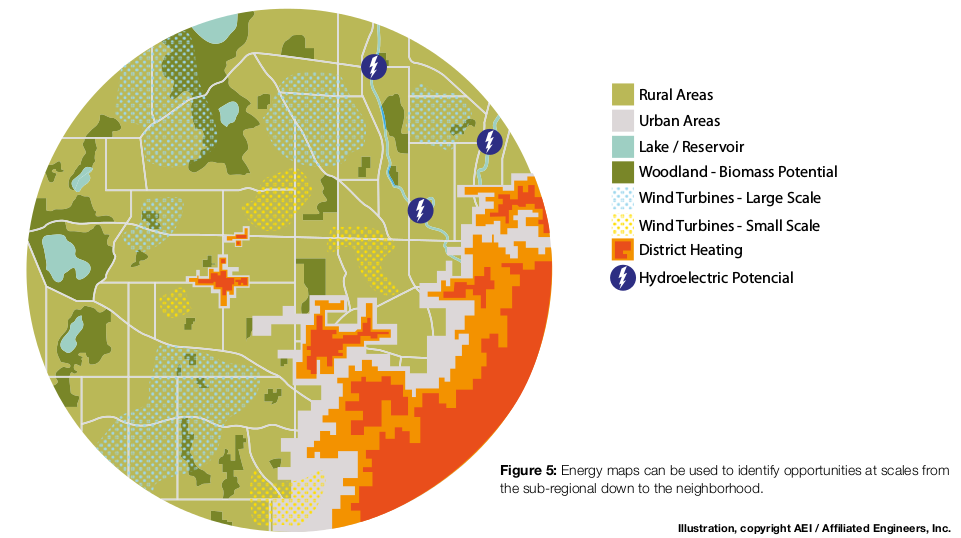
\includegraphics[width=0.7\linewidth]{energyMapIDEA.png}
  \caption{IDEA schematic energy map~\cite{IDEA2012}}
  \label{fig:energyMapIDEA}
\end{figure}

The work flow of the energy map creation and the information involved
in the process are as follows (adapted from \cite{IDEA2012})
\begin{enumerate}[{Step }1]
\item \textbf{Objective Setting}
  \begin{itemize}
  \item People;
  \item Planet;
  \item Profit;
  \end{itemize}
\item \textbf{Data collection}
  \begin{itemize}
  \item Energy Demand (hourly scale~\cite{Baird2014})
    \begin{itemize}
    \item Current energy consumption
    \item Future energy consumption
      \begin{itemize}
        \item new development rate
        \item improvement of building energy efficiency,
        \item improvement of people's energy use behavior
        \end{itemize}
      \end{itemize}
    \item Energy sources
      \begin{itemize}
      \item Renewable: solar, wind, geothermal, biomass, water body
      \end{itemize}
    \item Energy delivery system;
      \begin{itemize}
      \item Existing district network
      \end{itemize}
    \end{itemize}
  \item \textbf{Analysis}
    \begin{itemize}
    \item ``suitability of low carbon technology''~\cite{IDEA2012}
      \begin{itemize}
      \item Basic function
        \begin{itemize}
        \item Development scale
        \item Service area
        \item Energy supply profile
        \item ``Implications for phasing''~\cite{IDEA2012}
        \item Constraints: land use, zoning regulation etc.
        \end{itemize}
      \item People
      \item Planet
        \begin{itemize}
        \item Annual total $CO_2$ emission
        \item ``Ability to integrate local or renewable fuel
          sources.''~\cite{IDEA2012}
        \end{itemize}
      \item Profit
        \begin{itemize}
        \item cost, 
        \item profit,
        \item payback period.
        \end{itemize}
      \end{itemize}
    \item site analysis based on data from the previous step and land
      use constraint
    \end{itemize}
\end{enumerate}

From this analysis above, the current dynamic energy map has
information of ``Current energy consumption'' but lacks the other
information.
\newpage
\bibliographystyle{plain}
\bibliography{myCitation}
\end{document}